\section{Refinement-based game semantics}

This section introduces the category $\mathcal{G}$ of games and strategies
we use to interpret the behavior of low-level interacting components.
$\mathcal{G}$ has no high-order structure,
which simplifies the definition of games considerably.
On the other hand,
our definition of strategy is generalized to accomodate specifications,
and the morphisms of $\mathcal{G}$ are equipped with a notion of refinement
suitable for our purposes.

\subsection{Games} %{{{

\subsubsection{Elementary games} %{{{

The elementary games which underlie
our category of games and strategies
can be decribed in the following way.

\begin{definition} % elementary game {{{
An \emph{elementary game} is a pair
$A = \langle M_A^\kw{Q}, M_A^\kw{A} \rangle$, where
$M_A^\kw{Q}$ is a set of \emph{questions}, and
$M_A^\kw{A}$ is a set of \emph{answers}.
\end{definition}
%}}}

The game proceeds as follows:
$\kw{O}$ chooses a question, then
$\kw{P}$ chooses an answer.
Elementary games place no restrictions
on the valid plays,
but this can be specified relationally.

\begin{definition} % refinement convention {{{
A \emph{refinement convention} between elementary games $A_1$ and $A_2$
is a tuple
$\mathbb{C} = \langle W_\mathbb{C}, \preceq_\mathbb{C}^\kw{Q}, \preceq_\mathbb{C}^\kw{A} \rangle$
consisting in a set $W_\mathbb{C}$ of \emph{worlds},
and two relations
${\preceq}_\mathbb{C}^\kw{Q} : \mathcal{R}_{W_\mathbb{C}}(M_{A_1}^\kw{Q},M_{A_2}^\kw{Q})$ and
${\preceq}_\mathbb{C}^\kw{A} : \mathcal{R}_{W_\mathbb{C}}(M_{A_1}^\kw{A},M_{A_2}^\kw{A})$.
We write $\mathbb{C} : \mathcal{R}(A_1, A_2)$.
\end{definition}
%}}}

Refinement conventions specify a correspondance
between the questions and answers of their source and target games,
which can be extended to plays and strategies.
The use of worlds ensures that the question and answer
are related in a consistent way.
If the source and target are the same game,
this is can be used to specify a set of valid plays
and augment the game with a notion of refinement.

\begin{definition} % game with refinement {{{
A \emph{game with refinement} $\langle A, \preceq_A \rangle$
is an elementary game
$A = \langle M_A^\kw{Q}, M_A^\kw{A} \rangle$
together with a refinement convention
$\mathbb{C}_A = \langle W_{\!A}, {\preceq}_A^\kw{Q}, {\preceq}_A^\kw{A} \rangle
  : \mathcal{R}(A, A)$
such that $\preceq_A^\kw{Q}$ and $\preceq_A^\kw{R}$
are transitive at all worlds.
\end{definition}
%}}}

In the context of games with refinement,
the valid plays and strategies will be the ones
that are self-related.

Our focus will be the plays and strategies
for the composite game $A \rightarrow B$
described in \S\ref{sec:arrow}.
Before we formally define them,
we start by addressing
the possibility for $\kw{P}$ to silently diverge,
to signal an undefined behavior,
and to refuse any question from $\kw{O}$.

%}}}

\subsubsection{Divergence} %{{{

We model internal actions in the following way.
Whenever $\kw{P}$ is to play,
it may instead perform an internal action ($\tau$),
in which case $\kw{P}$ will retain control.
There is no limit on the number of internal actions that
$\kw{P}$ may perform before playing a move;
we say that a strategy \emph{diverges}
when it performs internal actions indefinitely.

Internal actions usually correspond to the hidden interactions
within composite systems, and
divergence is an \emph{emergent} phenomenon:
systems that are well-behaved when taken in isolation
may nontheless exhibit divergence when they interact with one another.
As such,
divergence is one of the major sources of complexity
in compositional semantics.

In our setting,
the occurence of internal actions
is observable,
and our definition of simulation
makes no effort
to identify finite sequences of internal actions
which have different lengths.
Instead,
in \S\ref{sec:bigstep}
we introduce an operator $- \backslash \tau^*$
that can be used to normalize strategies
by eliminating altogether all such finite sequences.

%}}}

\subsubsection{Undefined behaviors} %{{{

Low-level language semantics and specifications
often contain \emph{undefined behaviors}:
there are circumstances under which the behavior of the system
is entierly unrestricted;
any execution that reaches such circumstances is said to ``go wrong''.
We model this by allowing $\kw{P}$ to play the special move
$\lightning$
to signal an undefined behavior,
after which the game terminates.

The undefined behavior can be implemented by anything,
but can only implement itself;
as such,
the single-event trace $\lightning$
acts as an upper bound with respect to refinement.

%}}}

\subsubsection{Arrow games} %{{{
\label{sec:arrow}

The arrow game $A \rightarrow B$ consists of
nested iterations of the elementary games $A$ and $B$.
In instances of $A$, the roles of $\kw{P}$ and $\kw{O}$ are exchanged;
instances of $B$ proceed normally.
When a new instance is initiated,
the current game is suspended
until the new instance concludes.

Accounting for divergence ($\Delta$) and undefined behaviors ($\lightning$),
the valid plays of $A \rightarrow B$
are described by the graph:
\[
  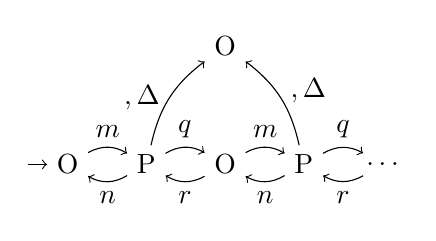
\begin{tikzpicture}[baseline=(O1.base)]
    \node (O1) at (0,0) {\kw{O}};
    \node (P1) at (1,0) {\kw{P}};
    \node (O2) at (2,0) {\kw{O}};
    \node (P2) at (3,0) {\kw{P}};
    \node (O3) at (4,0) {$\ldots$};
    \node (H) at (2,1.5) {\kw{O}};
    \path [->] (-0.5,0) edge (O1);
    \path [->] (O1) edge[bend left] node[auto] {$m$} (P1);
    \path [->] (P1) edge[bend left] node[auto] {$n$} (O1);
    \path [->] (P1) edge[bend left] node[auto] {$q$} (O2);
    \path [->] (P1) edge[bend left=20] node[auto,anchor=east] {$\lightning, \Delta$} (H);
    \path [->] (O2) edge[bend left] node[auto] {$r$} (P1);
    \path [->] (O2) edge[bend left] node[auto] {$m$} (P2);
    \path [->] (P2) edge[bend left] node[auto] {$n$} (O2);
    \path [->] (P2) edge[bend left] node[auto] {$q$} (O3);
    \path [->] (P2) edge[bend right=20] node[anchor=base west] {$\lightning, \Delta$} (H);
    \path [->] (O3) edge[bend left] node[auto] {$r$} (P2);
  \end{tikzpicture}
  \quad
  \begin{array}{c@{\,}lc@{\,}l}
    m &\in M_B^\kw{Q} & q &\in M_A^\kw{Q} \\[1ex]
    n &\in M_B^\kw{A} & r &\in M_A^\kw{A}
  \end{array}
\]
The first move is always a question $m$ played by $\kw{O}$ in $B$.
The player $\kw{P}$ can conclude the current instance of $B$
with an answer $n$, or
initiate an instance of $A$
with a question $q$.
Then $\kw{O}$ can initiate a new instance of $B$
with another $m$, or
conclude any current instance of $A$
with an answer $r$.
This process goes on indefinitely.

To formalize the plays and strategies of $A \rightarrow B$
in a way that accounts for refinement,
we decouple two aspects of this structure.
The following definition of plays
enforces the alternation between $\kw{O}$ and $\kw{P}$.

\begin{definition} % arrow game {{{
Given two elementary games $A$ and $B$,
the moves of the arrow game $A \rightarrow B$
are the questions and answers of $A$ and $B$,
categorized as follows:
\begin{align*}
  M_{A \rightarrow B}^\kw{O} &= M_A^\kw{A} + M_B^\kw{Q} &
  M_{A \rightarrow B}^\kw{Q} &= M_A^\kw{Q} + M_B^\kw{Q} \\
  M_{A \rightarrow B}^\kw{P} &= M_A^\kw{Q} + M_B^\kw{A} &
  M_{A \rightarrow B}^\kw{A} &= M_A^\kw{A} + M_B^\kw{A}
\end{align*}
The \emph{plays} are taken in
the prefix closure $P_{A \rightarrow B}$ of the set:
\[
    (M_{A \rightarrow B}^\kw{O}
     M_{A \rightarrow B}^\kw{P})^* \,
    (\varepsilon +
     M_{A \rightarrow B}^\kw{O} \Delta +
     M_{A \rightarrow B}^\kw{O} \lightning) \,.
\]
Note that
even-length plays represent positions where $\kw{O}$ is expected to play,
whereas odd-length plays represent positions where $\kw{P}$ is.
We write $P_{A \rightarrow B}^\kw{even}$ and $P_{A \rightarrow B}^\kw{odd}$
for the corresponding subsets of $P_{A \rightarrow B}$.
\end{definition}
%}}}

The ``stack discipline'' associating questions
with their eventual answer is captured by
the way we extend refinement conventions to
the plays of $A \rightarrow B$.

\begin{definition} % F_A->B %{{{
Given
$\mathbb{C}_A : \mathcal{R}(A_1, A_2)$ and
$\mathbb{C}_B : \mathcal{R}(B_1, B_2)$,
we can define the following relations
between the moves of $A_1 \rightarrow B_2$
and the moves of $A_2 \rightarrow B_2$:
\begin{align*}
  {\preceq}_{\mathbb{C}_A \rightarrow \mathbb{C}_B}^\kw{O} &=
    {\preceq}_{\mathbb{C}_A}^\kw{A} +
    {\preceq}_{\mathbb{C}_B}^\kw{Q} &
  {\preceq}_{\mathbb{C}_A \rightarrow \mathbb{C}_B}^\kw{Q} &=
    {\preceq}_{\mathbb{C}_A}^\kw{Q} +
    {\preceq}_{\mathbb{C}_B}^\kw{Q} \\
  {\preceq}_{\mathbb{C}_A \rightarrow \mathbb{C}_B}^\kw{P} &=
    {\preceq}_{\mathbb{C}_A}^\kw{Q} +
    {\preceq}_{\mathbb{C}_B}^\kw{A} &
  {\preceq}_{\mathbb{C}_A \rightarrow \mathbb{C}_B}^\kw{A} &=
    {\preceq}_{\mathbb{C}_A}^\kw{A} +
    {\preceq}_{\mathbb{C}_B}^\kw{A} \,,
\end{align*}
The Kripke frame
$\mathcal{F}_{\mathbb{C}_A \rightarrow \mathbb{C}_B} =
 \langle W_{\mathbb{C}_A \rightarrow \mathbb{C}_B}, \leadsto \rangle$
has worlds in
$W_{\mathbb{C}_A \rightarrow \mathbb{C}_B} =
 (W_{\mathbb{C}_A} + W_{\mathbb{C}_B})^*$,
and its accessibility relation $\leadsto$
relates moves of $A_1 \rightarrow B_1$
to moves of $A_2 \rightarrow B_2$,
as defined by the rules:
\[
    \AxiomC{$m_1 \ifr{w \Vdash {\preceq}_{\mathbb{C}_A \rightarrow \mathbb{C}_B}^\kw{Q}} m_2$}
    \UnaryInfC{$\vec{w} \stackrel{m_1, m_2}{\leadsto} w :: \vec{w}$}
    \DisplayProof
    \quad
    %\begin{array}{c}
    %  \vec{w} \stackrel{\#,\#}{\leadsto} \vec{w} \\[0.7ex]
    %  \vec{w} \stackrel{\tau, \tau}{\leadsto} \vec{w}
    %\end{array}
    %\quad
    \AxiomC{$m_1 \ifr{w \Vdash {\preceq}^\kw{A}_{\mathbb{C}_A \rightarrow \mathbb{C}_B}} m_2$}
    \UnaryInfC{$w :: \vec{w} \stackrel{m_1, m_2}{\leadsto} \vec{w} \,.$}
    \DisplayProof
\]
%Then two plays are related at $\vec{w}$
%when there is a path from $\varepsilon$ to $\vec{w}$
%in $\leadsto$ whose labels project onto the plays:
%\[
%    \AxiomC{$s : \varepsilon \leadsto^* \vec{w}$}
%    \UnaryInfC{$\pi_1^*(s)
%       \ifr{\vec{w} \Vdash {\preceq}_{A \rightarrow B}}
%       \pi_2^*(s)$}
%    \DisplayProof
%\]
%If
%$\langle A, \mathbb{C}_A \rangle$ and
%$\langle B, \mathbb{C}_B \rangle$
%are two games with refinement, then
%a \emph{valid play} of $A \rightarrow B$
%is a sequence $s \in P_{A \rightarrow B}$
%such that $(s, s) \in [\vec{w} \Vdash {\preceq}_{A \rightarrow B}]$
%for some $\vec{w}$.
\end{definition}

The frame $\mathcal{F}_{\mathbb{C}_A \rightarrow \mathbb{C}_B}$
is used in \S\ref{sec:sim}
to define our notion of simulation.
%}}}

%}}}

%}}}

\subsection{Behavior specifications} %{{{

By contrast with more traditional settings,
in our model strategies represent a range of possible behaviors
of the system and as such are not expected to be deterministic.
In addition,
our explicit treatment of divergence,
the possibility for strategies to exhibit undefined behaviors,
and our commitment to strategy refinement as a first-class citizen
[...]

In this section,
we capture these aspects of our model
in the \emph{behavior specification} monad.

\subsubsection{Definition}

Given a base type $A$,
a computation in $A$ may produce 
may produce a value of type $A$,
but it may also diverge or exhibit undefined behavior.
Hence,
a behavior specification for $A$ is an element:
\[
    x \in \mathcal{B}(A) = \mathcal{P}(A + \{ \Delta, \lightning \})
\]
The unit of $\kw{ret}_A : A \rightarrow \mathcal{B}(A)$
of the monad $\mathcal{B}$ is given by:
\[
    \kw{ret}_A(a) = \{ a \} \,,
\]
and the binding operation is defined in the following way:
\[
    \AxiomC{$a \in x$}
    \AxiomC{$b \in f(a)$}
    \BinaryInfC{$b \in x >>= f$}
    \DisplayProof
    \quad
    \AxiomC{$\Delta \in x$}
    \UnaryInfC{$\Delta \in x >>= f$}
    \DisplayProof
    \quad
    \AxiomC{$\lightning \in x$}
    \UnaryInfC{$\lightning \in x >>= f$}
    \DisplayProof
\]
The usual monad laws hold, and
the Kleisi composition of $f : A \rightarrow \mathcal{B}(B)$ and
$g : B \rightarrow \mathcal{B}(C)$ can be derived as:
\[
    (f \cdot g)(a) = (f(a) >>= g) \,.
\]
The action of $\mathcal{B}$ on functions can be derived as:
\[
    \mathcal{B}(f) = x \mapsto (x >>= \kw{ret}_A \circ f) \,.
\]


\subsubsection{Refinement}

We can promote a relation $R : \mathcal{R}(A, B)$
to behavior specifications as:
\[ \mathcal{B}^+(R) :=
   \mathcal{P}^+(R + \{ (\Delta, \Delta), (x, \lightning) \mid x \in A \}) \]
Note that $\mathcal{B}$ preserves reflexivity and transitivity,
so that if $\sqsubseteq$ is a preorder,
then $\mathcal{B}(\sqsubseteq)$ is a preorder as well.

The least and greatest elements
can be defined as:
\[ \bot := \varnothing \qquad \top := \{ \lightning \} \,, \]
with the property that for all $R, x, S$:
\[ \bot \ifr{\mathcal{B}^+(R)} x \ifr{\mathcal{B}^+(S)} \top \,. \]

In addition,
for $R : \mathcal{R}(A_1, A_2)$ and $S : \mathcal{R}(B_1, B_2)$,
the monad operations satisfy the expected relational properties:
\begin{gather*}
\kw{ret}_{A_1} \ifr{R \rightarrow \mathcal{B}^+(R)} \kw{ret}_{A_2} \\
({>>=}) \ifr{\mathcal{B}^+(R) \rightarrow (R \rightarrow \mathcal{B}^+(S))
  \rightarrow \mathcal{B}^+(S)} ({>>=}) \\
{\cdot} \ifr{(R \rightarrow \mathcal{B}^+(S)) \rightarrow
             (S \rightarrow \mathcal{B}^+(T)) \rightarrow
             (R \rightarrow \mathcal{B}^+(T))} {\cdot} \\
\mathcal{B}(-) \ifr{(R \rightarrow S) \rightarrow (\mathcal{B}^+(R)
\rightarrow \mathcal{B}^+(S))} \mathcal{B}(-)
\end{gather*}

\subsubsection{Kleene star}

A Kleisli morphism of type $f : A \rightarrow \mathcal{B}(A)$
can be interpreted as a transition relation on the set of states $A$,
and we can define the iteration $f^*$
in a way that recognizes silent divergence.
Writing $f^n$ for the $n$-fold composition of the form
$f \cdot f \cdots f$,
divergence can be recognized as:
\[ \kw{diverges}_f(a) \Leftrightarrow
    \forall n \in \mathbb{N} \,.\,
    \exists a' \in A \,.\,
    f^n(a) \ni a' \]
Nondeterministic choice
and its unit can be defined as:
\[ f + g := a \mapsto f(a) \cup g(a)  \qquad  0 := a \mapsto \bot \]
Then the iteration of $f$ is:
\[ f^* := \sum_{n \in \mathbb{N}} f^n +
          (a \mapsto \{ \Delta \mid \kw{diverges_f(a)} \}) \]

Using Kleisi composition as multiplication,
the structure
$\langle A \rightarrow \mathcal{B}(A), {\cdot}, {+}, \kw{ret}_A, 0, * \rangle$
is analogous to a Kleene algebra.
However, as noted in \cite{failkat},
the possibility of an abnormal outcome
means that annihilation of $\cdot$ by $0$ on the right
does not hold.
In particular:
\[ \Delta \cdot 0 = \Delta \qquad \lightning \cdot 0 = \lightning \]

Nevertheless,
this notion of iteration
and the associated equational theory
will be useful
for defining strategies operationally,
in terms of small-step transition relations.

%}}}

\subsection{Strategies} %{{{

A strategy for $A \rightarrow B$
is essentially a tree
which gathers the possible interactions of
the system being modeled.
We give a traditional representation
as a prefix-closed set of plays,
but will work with strategies defined as transition systems.

\subsubsection{Traces} %{{{

In the existing literature,
strategies are usually formalized as prefix-closed sets of plays.
This establishes a connection with trace semantics of process calculi.
In our case,
a strategy given in this form is a set:
\[ \sigma \subseteq P_{A \rightarrow B} \,, \]
which satisfies
for all $st \in P_{A \rightarrow B}$
and $m \in M_{A \rightarrow B}^\kw{O}$:
\begin{itemize}
  \item $st \in \sigma \Rightarrow s \in \sigma$;
  \item $s \in \sigma \wedge sm \in P_{A \rightarrow B}
    \Rightarrow sm \in \sigma$.
\end{itemize}
The first condition ensures that $\sigma$ is prefix-closed,
whereas the second condition ensures that
all possible behaviors of $\kw{O}$ are included
at all reachable positions.

XXX require downward closure wrt $\lightning$
so that unique and ordered by inclusion.

%}}}

\subsubsection{Transition systems} %{{{

Instead of manipulating sets of traces directly,
we will define strategies using a specialized form of transition system.

\begin{definition} % strategy {{{
\label{def:strat}
An \emph{strategy} $\sigma$ for the arrow game $A \rightarrow B$
is a tuple
$\langle K, S,
{\xrightarrow{\kw{O}} },
{\xrightarrow{\tau}},
{\xrightarrow{\kw{P}} },
 \#, k_0 \rangle$
where:
\begin{itemize}
  \item $K$ is a set of \emph{continuation states};
  \item $S$ is a set of \emph{running states};
  \item ${\stackrel{\kw{O}}{\rightarrow}} :
         K \rightarrow
         M_{A \rightarrow B}^\kw{O} \rightarrow
         \mathcal{P}(S^\lightning)$
    is a \emph{resumption relation};
  \item ${\stackrel{\tau}{\rightarrow}} :
         S \rightarrow \mathcal{P}(S^\lightning)$
    is an \emph{internal transition relation};
  \item ${\stackrel{\kw{P}}{\rightarrow}} :
         S \rightarrow \mathcal{P}(M_{A \rightarrow B}^\kw{P} \times K)$
    is a \emph{suspension relation};
  \item ${\#} : K \rightarrow \mathcal{P}(M_B^\kw{Q})$
    is a \emph{refusal relation};
  \item $k_0$
    is the strategy's \emph{initial continuation}.
\end{itemize}
The set of states is extended to $S^\lightning = S \uplus \{\lightning\}$
so that $\sigma$ may perform a transition to $\lightning$
whenever an undefined behavior is encountered.
We will write:
\begin{itemize}
  \item $k \xrightarrow{m} s$ when ${\xrightarrow{\kw{O}} }(k, m) \ni s$, and
  \item $s \xrightarrow{m} k$ when ${\xrightarrow{\kw{P}} }(s) \ni (m, k)$.
\end{itemize}
We write $\sigma : A \rightarrow B$ when $\sigma$ is a strategy
for $A \rightarrow B$.
\end{definition}
%}}}

Continuations correspond to
the points in the execution where $\kw{O}$ is expected to move,
whereas states correspond to
the points where $\kw{P}$ is expected to move.
The set of traces associated with a state is
defined by mutual recursion as:
\[
  \begin{array}{l@{\:}c@{\:\{}l@{\:\mid\:}l}
    \kw{traces}_\sigma(k) & = & \varepsilon, m &
      m \in M_{A \rightarrow B}^\kw{O} \} \\
    & \cup & m t &
      k \xrightarrow{m} s \wedge t \in \kw{traces}_\sigma(s) \} \\
    & \cup & m \# &
      k \: \# \: m \} \\
    \kw{traces}_\sigma(s) & = & \tau, \tau t &
      s \xrightarrow{\tau} s' \wedge t \in \kw{traces}_\sigma(s') \} \\
    & \cup & m t &
      s \xrightarrow{m} k \wedge t \in \kw{traces}_\sigma(k) \} \\
    & \cup & \lightning & s = \lightning \}
  \end{array}
\]
Then the behavior of strategies can be made explicit
by specifying the corresponding sets of plays as:
\[
  \kw{traces}(\sigma) = \kw{traces}_\sigma(k_0) \,.
\]

XXX downward closure wrt $\lightning$

[Show that $\subseteq P_{A \rightarrow B}$,
and that it satisfies the requirements outlined
in the previous section.]

[Advantages: alternation structure baked in,
can be handled by the proof assistant's type system.
Facilitates embedding of operational semantics,
and intuitive operational reasoning.]

[Inconvenient: junk and non unique,
but we don't care because we're going to
define simulations and quotient anyway.]

%}}}

%}}}

\subsection{Simulations} %{{{
\label{sec:sim}

Having formally defined a notion of strategy
for the game $A \rightarrow B$,
we turn to the corresponding relational notion of simulation
for the refinement convention $\mathbb{C}_A \rightarrow \mathbb{C}_B$.
To this end,
we first introduce the following modal constructions.

\begin{definition} % modal relators for simulation {{{
For frames labelled by pairs
($\Lambda = \Lambda_1 \times \Lambda_2$),
we define variants of $\Box, \Diamond$ which
allow world transitions to interact with the components
being related.
The relators:
\begin{align*}
  \Diamond \times {-} &: \mathcal{R}_W(A, B) \rightarrow
              \mathcal{R}_W(\Lambda_1 \times A, \, \Lambda_2 \times B) \\
  \Box \rightarrow - &: \mathcal{R}_W(A, B) \rightarrow
          \mathcal{R}_W(\Lambda_1 \rightarrow A, \, \Lambda_2 \rightarrow B) \\
  \mathcal{P}^+(\Box) &:
      \mathcal{R}_W(\mathcal{P}(\Lambda_1), \mathcal{P}(\Lambda_2))
\end{align*}
are defined as:
\begin{gather*}
  (l_1, a) \ifr{w \Vdash \Diamond \times R} (l_2, b) \Leftrightarrow
    a \ifr{w \Vdash \langle l_1, l_2 \rangle R} b \\
  f \ifr{w \Vdash \Box \rightarrow R} g \Leftrightarrow
    \forall \, l_1 l_2 \,.\, f(l_1) \ifr{w \Vdash [l_1, l_2] R} g(l_2) \\
  L_1 \ifr{w \Vdash \mathcal{P}^+(\Box)} L_2 \Leftrightarrow
    \forall \, w \stackrel{l_1, l_2}{\leadsto} w' \,.\,
      l_1 \in L_1 \Rightarrow l_2 \in L_2 \,.
\end{gather*}
\end{definition}
%}}}

With these constructions,
our notion of simulation relation
is naturally derived from
the types we used to define strategies (Def.~\ref{def:strat}).
They are used
with respect to the frame $\mathcal{F}_{A \rightarrow B}$
defined in \S\ref{sec:arrow}.
Hence, the simulation operates in the context of
a stack of elementary worlds
specifying how answers to pending questions
should be related.
In each one of the component games $A_i$ and $B_i$,
answers will be related at the same world as the corresponding questions:
$\kw{P}$ can rely on $\kw{O}$ making this true for $A$;
it must guarantee that this is true for $B$.

\begin{definition} % simulation relation {{{
Given
$\mathbb{C}_A : \mathcal{R}(A_1, A_2)$,
$\mathbb{C}_B : \mathcal{R}(B_1, B_2)$
two refinement conventions, and
$\sigma_1 : A_1 \rightarrow B_1$,
$\sigma_2 : A_2 \rightarrow B_2$
two strategies,
a \emph{simulation relation} between $\sigma_1$ and $\sigma_2$
is a pair of relations $R = \langle R_S, R_K \rangle$ with
$R_K : \mathcal{R}_{W_{\!A \rightarrow B}}(K_1, K_2)$ and
$R_S : \mathcal{R}_{W_{\!A \rightarrow B}}(S_1, S_2)$
such that:
\begin{gather*}
  \xrightarrow{\kw{O}}_1
  \ifr{\Vdash R_K \rightarrow \Box \rightarrow \mathcal{P}^+(R_S^\lightning)}
  \xrightarrow{\kw{O}}_2
  \\
  \xrightarrow{\tau}_1
  \ifr{\Vdash R_S \rightarrow \mathcal{P}^+(R_S^\lightning)}
  \xrightarrow{\tau}_2
  \\
  \xrightarrow{\kw{P}}_1
  \ifr{\Vdash R_S \rightarrow \mathcal{P}^+(\Diamond \times R_K)}
  \xrightarrow{\kw{P}}_2
  \\
  \#_1
  \ifr{\Vdash R_K \rightarrow \Box \rightarrow {\Rightarrow}}
  \#_2
  \\
  k_{0,1} \ifr{\varepsilon \Vdash R_K} k_{0,2}
\end{gather*}
The relation on states is extended to:
\[
    R_S^\lightning =
    R_S \cup \{ (s_1, \lightning) \mid s_1 \in S_1^\lightning \} \,.
\]
We will write
$\sigma_1 \le_{\mathbb{C}_A \rightarrow \mathbb{C}_B}^R \sigma_2$
when $R$ is a simulation relation in this sense, and write
$\sigma_1 \le_{\mathbb{C}_A \rightarrow \mathbb{C}_B} \sigma_2$
when there exists any such simulation relation.
\end{definition}
%}}}

%}}}

\subsection{Operators} %{{{

\subsubsection{Multi-component games and strategies} %{{{

The simplest way to aggregate a family of strategies $(\sigma_i)_{i\in I}$
is to annotate all of the moves exchanged by the system with its environment
by a component identifier $i$.

\begin{definition} % multi-channel game {{{
For an elementary game $A$ and a set $I$,
we define the \emph{multi-channel game}
$A^I = \langle I \times M_G^\kw{Q}, I \times M_G^\kw{A} \rangle$.
Given a refinement convention
$\mathbb{C} : \mathcal{R}(A_1, A_2)$,
we define
$\mathbb{C}^I =
 \langle W, {\preceq}^\kw{Q}, {\preceq}^\kw{A} \rangle :
 \mathcal{R}(A_1^I, A_2^I)$
where
$W = I \times W_\mathbb{C}$ and
$\preceq^\kw{Q}, \preceq^\kw{A}$
are given by the rules:
\[
    \small
    \AxiomC{$m_1 \ifr{w \Vdash {\preceq}_\mathbb{C}^\kw{Q}} m_2$}
    \UnaryInfC{$(i, m_1) \ifr{(i, w) \Vdash {\preceq}^\kw{Q}} (i, m_2)$}
    \DisplayProof
    \quad
    \AxiomC{$m_1 \ifr{w \Vdash {\preceq}_\mathbb{C}^\kw{A}} m_2$}
    \UnaryInfC{$(i, m_1) \ifr{(i, w) \Vdash {\preceq}^\kw{A}} (i, m_2)$}
    \DisplayProof
\]
\end{definition}
%}}}

The aggregated strategy uses the labels to direct each move
to the corresponding component,
and lets the components operate independently.

\begin{definition} % multi-component strategy {{{
For a family of strategies
$\vec{\sigma} = (\sigma_i)_{i \in I}$
with
$\sigma_i = \langle K_i, S_i, \xrightarrow{\kw{O}}_i,
  \xrightarrow{\tau}_i, \xrightarrow{\kw{P}}_i, \#_i, k_{0i} \rangle :
  A \rightarrow B$,
the multi-component strategy
$\mathcal{M}(\sigma_i)_{i \in I} : A^I \rightarrow B^I$
is defined over the sets of states:
\[
  K := \prod_{i \in I} K_i \qquad
  S := \sum_{i \in I}
    \Big( S_i \times \prod_{i \ne j} K_j \Big)
\]
by the following rules:
\[
  \begin{array}{c@{\qquad}c}
    \AxiomC{$k_i \xrightarrow{m}_i s$}
    \UnaryInfC{$\vec{k} \xrightarrow{(i, m)} (i, s, \vec{k} \backslash i)$}
    \DisplayProof
    &
    \AxiomC{$s \xrightarrow{m}_i k_i$}
    \UnaryInfC{$(i, s, \vec{k} \backslash i) \xrightarrow{(i, m)} \vec{k}$}
    \DisplayProof
    \\[1.5em]
    \AxiomC{$s \xrightarrow{\tau}_i s'$}
    \UnaryInfC{$(i, s, \vec{k}) \xrightarrow{\tau} (i, s', \vec{k})$}
    \DisplayProof
    &
    \AxiomC{$k \: \#_i \: m$}
    \UnaryInfC{$\vec{k} \: \# \: (i, m)$}
    \DisplayProof
  \end{array}
\]
and uses the initial continuation $(k_{0i})_{i \in I}$.
\end{definition}
%}}}

In other words,
at most one component is active at any time,
and the others remain in continuation states.
A resumption activates the component whose index
is read from the move,
and the index is incoroporated back into
any move played by the component.

\begin{lemma} % monotonicity {{{
For a family of simulation relations $\vec{R} = (R_i)_{i \in I}$ such that
$\sigma_{1,i} \le_{\mathbb{C}_A \rightarrow \mathbb{C}_B}^{R_i} \sigma_{2,i}$,
the relation $\mathcal{M}(\vec{R})$ defined by:
\begin{gather*}
  \AxiomC{$\forall i \,.\,
    k_{1,i} \ifr{\vec{w} \restriction i \Vdash R_{K,i}} k_{2,i}$}
  \UnaryInfC{$\vec{k_1} \ifr{\vec{w} \Vdash \mathcal{M}(\vec{R})_K} \vec{k_2}$}
  \DisplayProof
  \\[.5ex]
  \AxiomC{$s_1 \ifr{\vec{w} \restriction i \Vdash R_{S,i}} s_2$}
  \AxiomC{$\forall j \ne i \,.\,
    k_{1,j} \ifr{\vec{w} \restriction j \Vdash R_{S,j}} k_{2,j}$}
  \BinaryInfC{$(i, s_1, \vec{k}_1)
    \ifr{\vec{w} \Vdash \mathcal{M}(\vec{R})_S}
    (i, s_2, \vec{k}_2)$}
  \DisplayProof
\end{gather*}
is a simulation relation between the strategies:
\[
  \mathcal{M}(\vec{\sigma_1})
  \le_{\mathbb{C}_A^I \rightarrow \mathbb{C}_B^I}^{\mathcal{M}(\vec{R})}
  \mathcal{M}(\vec{\sigma_2}) \, .
\]
The stack of worlds $\vec{w} \restriction i$
is the sequence $w_1, w_2, \ldots, w_n$
such that $(i, w_1), (i, w_2), \ldots, (i, w_n)$
is the subsequence of $\vec{w}$ containing worlds
paired with $i$ indices.
\end{lemma}
%}}}

%}}}

\subsubsection{Flat composition} %{{{

Once we have such an aggregate,
we can ``flatten'' the communication between
the system and the environment
back to the unannotated game $A \rightarrow B$.

\begin{definition} % flattening {{{
The \emph{flattening} of $\sigma : A^I \rightarrow B^I$
is the strategy $\sigma^\rhd : A \rightarrow B$
defined over the sets of states
$K := K_\sigma \times I^*$ and
$S := S_\sigma \times I^*$ by the following rules:
\[
  \begin{array}{c@{\quad}c}
    \AxiomC{$k \xrightarrow{(i, m)}_\sigma s$}
    \AxiomC{$\forall \, j \ne i \,.\, k \: \#_{\!\sigma} \: (j, m)$}
    \BinaryInfC{$(k, \iota) \xrightarrow{m} (s, \iota)$}
    \DisplayProof
    &
    \AxiomC{$s \xrightarrow{(i, n)}_\sigma k$}
    \UnaryInfC{$(s, \iota) \xrightarrow{n} (k, \iota)$}
    \DisplayProof
    \\[1.5em]
    \AxiomC{$s \xrightarrow{(i, q)}_\sigma k$}
    \UnaryInfC{$(s, \iota) \xrightarrow{q} (k, i :: \iota)$}
    \DisplayProof
    &
    \AxiomC{$k \xrightarrow{(i, r)}_\sigma s$}
    \UnaryInfC{$(k, i :: \iota) \xrightarrow{r} (s, \iota)$}
    \DisplayProof
    \\[1.5em]
    \AxiomC{$s \xrightarrow{\tau}_\sigma s'$}
    \UnaryInfC{$(s, \iota) \xrightarrow{\tau} (s', \iota)$}
    \DisplayProof
    &
    \AxiomC{$\forall \,i\,.\, k \: \#_{\!\sigma} \: (i, m)$}
    \UnaryInfC{$(k, \iota) \:\#\: m$}
    \DisplayProof
  \end{array}
\]
\end{definition}
%}}}

We direct an incoming question in $B$
to a component $i$ when all other components reject it.
If the component then asks a question in the game $A$,
we save its identifier on the stack $\iota$,
so that the corresponding answer can be directed back to $i$.

\begin{lemma}
Given a simulation relation
$\sigma_1 \le_{\mathbb{C}_A^I \rightarrow \mathbb{C}_B^I}^R \sigma_2$,
the relation $R^\rhd$ is defined for continuation states by:
\[
  \AxiomC{$k_1 \ifr{\vec{w} \Vdash R_K} k_2$}
  \AxiomC{$\iota = \pi_1^*(\vec{w}) \mbox{ XXX}$}
  \BinaryInfC{
    $(k_1, \iota) \ifr{\pi_2^*(\vec{w}) \Vdash R^\rhd_K} (k_2, \iota)$}
  \DisplayProof
\]
and similarly for running states.
$R^\rhd$ is a simulation relation:
\[
    \sigma_1^\rhd
    \le_{\mathbb{C}_A \rightarrow \mathbb{C}_B}^{R^\rhd}
    \sigma_2^\rhd \,.
\]
\end{lemma}

Putting together multi-component strategies and flattening,
the \emph{flat composition} operator
$\mathcal{F} : [A \rightarrow B] \rightarrow [A \rightarrow B]$
is:
\[
    \mathcal{F}(\vec{\sigma}) := \mathcal{M}(\vec{\sigma})^\rhd
\]
This allows us to bundle multiple components of the same type,
however note that so far they do not interact with each other
(only to decide who's going to handle what question).

%}}}

\subsubsection{Resolution operator} %{{{

To allow interaction within a composite system,
we define the following resolution operator,
which feeds back a strategy's own questions to itself
whenever possible.

\begin{definition} % resolution {{{
The \emph{resolution} of $\sigma : A \rightarrow A$,
written $\mathcal{R}(\sigma)$,
is defined over the sets of states
$K := K_\sigma \times \{\kw{O}, \kw{P}\}^*$ and
$S := S_\sigma \times \{\kw{O}, \kw{P}\}^*$
by the following rules:
\[
  \begin{array}{cc}
    {\small m \in M_A^\kw{Q}, \:\: n \in M_A^\kw{A}}
    &
    {\small q \in M_A^\kw{Q}, \:\: r \in M_A^\kw{A}}
    \\[1em]
    \AxiomC{$k \xrightarrow{m}_\sigma s$}
    \UnaryInfC{$(k, \iota) \xrightarrow{m} (s, \kw{O} :: \iota)$}
    \DisplayProof
    &
    \AxiomC{$s \xrightarrow{n}_\sigma k$}
    \UnaryInfC{$(s, \kw{O} :: \iota) \xrightarrow{n} (k, \iota)$}
    \DisplayProof
    \\[1.5em]
    \AxiomC{$s \xrightarrow{q}_\sigma k$}
    \AxiomC{$k \:\#_{\!\sigma}\: q$}
    \BinaryInfC{$(s, \iota) \xrightarrow{q} (k, \iota)$}
    \DisplayProof
    &
    \AxiomC{$k \xrightarrow{r}_\sigma s$}
    \UnaryInfC{$(k, \iota) \xrightarrow{r} (s, \iota)$}
    \DisplayProof
    \\[1.5em]
    \AxiomC{$s \xrightarrow{q}_\sigma k$}
    \AxiomC{$k \xrightarrow{q}_\sigma s'$}
    \BinaryInfC{$(s, \iota) \xrightarrow{\tau} (s', \kw{P} :: \iota)$}
    \DisplayProof
    &
    \AxiomC{$s \xrightarrow{r}_\sigma k$}
    \AxiomC{$k \xrightarrow{r}_\sigma s'$}
    \BinaryInfC{$(s, \kw{P} :: \iota) \xrightarrow{\tau} (s', \iota)$}
    \DisplayProof
    \\[1.5em]
    \AxiomC{$s \xrightarrow{\tau}_\sigma s'$}
    \UnaryInfC{$(s, \iota) \xrightarrow{\tau} (s', \iota)$}
    \DisplayProof
    &
    \AxiomC{$k \:\#_{\!\sigma}\: m$}
    \UnaryInfC{$(k, \iota) \:\#\: m$}
    \DisplayProof
  \end{array}
\]
The initial continuation is $(k_{\sigma}, \varepsilon)$.
\end{definition}
%}}}

\begin{lemma}
If
$\sigma_1 \le_{\mathbb{C}_A \rightarrow \mathbb{C}_A}^R \sigma_2$,
then
$\mathcal{R}(\sigma_1)
 \le_{\mathbb{C}_A \rightarrow \mathbb{C}_A}^{\mathcal{R}(R)}
 \mathcal{R}(\sigma_2)$,
where $\mathcal{R}(R)$ is defined as follows.
For a world $\vec{w} \in W_{A \rightarrow B}$
and a stack $\iota \in \{\kw{O}, \kw{P}\}^*$,
the set $\mathcal{R}_\iota(\vec{w}) \subseteq W_{A \rightarrow B}$
is defined by the following rules together with the base case
$\varepsilon \in \mathcal{R}_\varepsilon(\varepsilon)$:
\[
    \AxiomC{$\vec{w}' \in \mathcal{R}_\iota(\vec{w})$}
    \UnaryInfC{$x :: \vec{w}' \in \mathcal{R}_{\kw{O} :: \iota}(x :: \vec{w})$}
    \DisplayProof
    \quad
    \AxiomC{$\vec{w}' \in \mathcal{R}_\iota(\vec{w})$}
    \UnaryInfC{$x :: x :: \vec{w}' \in \mathcal{R}_{\kw{P} :: \iota}(\vec{w})$}
    \DisplayProof
\]
XXX this is only the rules for codomain worlds,
we need a case for domain worlds to be passed along.

Then the relation $\mathcal{R}(R)$ is given for continuation states by:
\[
  \AxiomC{$k_1 \ifr{\vec{w} \Vdash R_K} k_2$}
  \AxiomC{$\vec{w}' \in \mathcal{R}_\iota(\vec{w})$}
  \BinaryInfC{$(k_1, \iota) \ifr{\vec{w}' \Vdash \mathcal{R}(R)_K} (k_2, \iota)$}
  \DisplayProof
\]
and similarly for running states.

XXX the proof needs $\mathcal{R}(\vec{w})$ to take into account
whether the component is currently running (states) or not (continuations).
\end{lemma}

%}}}

\subsubsection{Observation operator} %{{{

The simulations defined in \S\ref{sec:sim}
only relate strategies whose internal actions match one-to-one.
However, the operator defined in this section
will allow us to normalize strategies by removing
all finite sequences of $\tau$s.

\begin{definition}
Given $\sigma : A \rightarrow B$,
the \emph{observation strategy}
$\sigma \backslash \tau^* =
 \langle K_\sigma, S_\sigma \uplus \{\ast\},
         \xrightarrow{\kw{O}},
         \xrightarrow{\tau},
         \xrightarrow{\kw{P}}_\sigma,
         \#_\sigma, k_{0,\sigma} \rangle$
uses the resumption and internal transition relations
defined by the rules:
\[
  \AxiomC{$s \xrightarrow{\tau}_\sigma s'$}
  \AxiomC{$s' \xrightarrow{\tau^\omega}$}
  \doubleLine \BinaryInfC{$s \xrightarrow{\tau^\omega}$}
  \DisplayProof
  \qquad
  \AxiomC{$k \xrightarrow{m}_\sigma s$}
  \AxiomC{$s \xrightarrow{\tau^\omega}$}
  \BinaryInfC{$k \xrightarrow{m} \ast$}
  \DisplayProof
\]\[
  \AxiomC{$k \xrightarrow{m}_\sigma s$}
  \AxiomC{$s \xrightarrow{\tau^*}_\sigma s' \xrightarrow{n}_\sigma k'$}
  \BinaryInfC{$k \xrightarrow{m} s'$}
  \DisplayProof
  \qquad
  \ast \xrightarrow{\tau} \ast \,.
\]
\end{definition}

\begin{lemma}
If $\sigma_1 \le_{\mathbb{C}_A \rightarrow \mathbb{C}_B}^R \sigma_2$,
then for $R \backslash \tau^* = R \cup \{(\ast, \ast)\}$
the following holds:
\[
  \sigma_1 \backslash \tau^*
  \le_{\mathbb{C}_A \rightarrow \mathbb{C}_B}^{R \backslash \tau^*}
  \sigma_2 \backslash \tau^* \,.
\]
\end{lemma}

%}}}

%}}}

{ \color{gray}
Note that for both states and continuations,
nondeterminism is interpreted as \emph{output} nondeterminism,
as prescribed by the use of the relator $\mathcal{P}^+$.
This means that alternating transition system
implicitely accept all possible inputs from the environment,
although some of them may cause the system to immediately go wrong.
Likewise,
the special resumption $\kw{refuse}$
is taken as a positive, output behavior from the system,
rather than a restriction on the environment ---
this will be important to establish the monotonicity
of the composition operator defined in Sec.~\ref{?}.
This approach corresponds to the saturation requirement on strategies
often found in traditional game semantics,
or notions of receptiveness used in CompCert
and in concurrency theory.

Furthermore, we need to distinguish between mere nondeterminism
and \emph{branching}.
This is explored in the following section.

\subsection{Branching and determinism}

Whereas nondeterminism allows a strategy to posess
multiple observable behaviors,
branching occurs when multiple state transitions
are associated with the same immediate observable behavior.
This can create spurious distinctions,
whereby systems that yield the same sets of traces
cannot be identified by simulation,
and as such we consider it undesirable.
The following definition
formalizes the conditions a transition system must satisfy
to be considered free from branching.

\begin{definition}[Nonbranching transition system]
For given sets of moves and states,
a continuation $k : M \rightarrow \mathcal{P}(\kw{resumption}(S))$
is \emph{nonbranching} if the following property holds:
\[ \forall m \,.\, | k(m) | \le 1 \]
A transition system $\alpha : \kw{ats}(M, S)$ is nonbranching
if the following property holds:
\[ \forall s, m, k_1, k_2 \,.\,
     \alpha(s) \supseteq \{ m \cdot k_1, m \cdot k_2 \} \Rightarrow
     k_1 = k_2 \,, \]
and if for all $s, m, k$ such that $\alpha(s) \ni \underline{m} \cdot k$,
the continuation $k$ is nonbranching.
\end{definition}

Determinism is a stronger property,
and ensures that the system has at most one possible behavior
at any point.
We expect the semantics of concrete systems ---
as opposed to specifications ---
to be deterministic in the following sense.

\begin{definition}[Deterministic transition system]
For given sets of moves and states,
a transition system $\alpha : \kw{ats}(M, S)$
is deterministic if for all $s$, $|\alpha(s)| \le 1$,
and if for all $s, m, k$ such that $\alpha(s) \ni \underline{m} \cdot k$,
the continuation $k$ is nonbranching.
\end{definition}

Note that both nonbranching and determinism
only relate to the behavior of the system.
In both cases,
the environment remains free to play any move.
Abramsky notes in \cite{cspgs}
that [it's one of the good things about game semantics].

\subsection{Internal actions and divergence}

The emergence of silent divergence
is one of the major difficulties
associated with modeling interacting systems.
Indeed,
two systems which, taken in isolation,
only exhibit reactive behavior,
can nonetheless become silently divergent when composed together,
if it is possible to interact with each other continuously
without intervening communication with the outside.

An operational description of this phenomenon
models this internal interaction explicitly
in the form of silent actions $\tau$.
When comparing the behavior of two systems,
finite sequences of $\tau$'s will be considered equivalent.
However,
silent divergence in the form of an infinite sequence of $\tau$'s
can only correspond to another infinite sequence.
This is usually addressed by the introduction of
sophisticated notions of simulation,
such as the \emph{measure simulations} used for instance in CompCert.

On the other hand,
in most work on denotational semantics,
including traditional game semantics such as \cite{pcfgs},
[complicated fixpoints] 

Our model includes a notion of internal action $\tau$,
which makes it possible to handle silent divergence explicitely
rather than through sophisticated domain-theoretic constructions.
However,
note that the notion of simulation we have defined
does not allow any variation
in the number of internal transitions
between the two transition systems being related.
Nevertheless,
composition operators remain monotonic
under this definition of simulation,
because [...]
Normalize using the following operator.

\begin{definition}[Observation operator]
For a transition system $\alpha : \kw{ats}(M, S)$,
we define the \emph{observations} transition system
$\mathcal{O}(\alpha)$ as follows.
A behavior $r : \kw{behavior}(M, S)$ is said to be
\emph{observable} if $r \ne \tau \cdot s$ for all $s \in S$.
A state $s' \in S$ is said to be \emph{reachable} from $s \in S$
if there is a sequence $s_0, s_1, \ldots s_n$ such that
$s_0 = s$, $s_n = s'$,
and for all $0 \le i < n$
there is a transition $\alpha(s_i) \ni \tau \cdot s_{i+1}$.
A state $s$ is said to be \emph{silently divergent}
if there is an infinite sequence $s_0, s_1, \ldots$
such that $s_0 = s$ and for all $i$,
there is a transition $\alpha(s_i) \ni \tau \cdot s_{i+1}$.
Then the observations transition system is defined as:
\begin{align*}
    \mathcal{O}(\alpha)(s) = &\{ r \:|\: r \mbox{ is observable } \wedge
         \exists s' \,.\, s \rightarrow^* s' \wedge
		\alpha(s') \ni r \} \\
      \cup &\{ \Delta \:|\: s \mbox{ is silently divergent} \}
\end{align*}
\end{definition}

Properties:
preserve nonbranching (if that's defined in the right way), determinism.
Monotonic.

}
